\chapter{Das Framework TensorFlow}

\gls{TF} ist eine plattformunabhängige Bibliothek für \gls{ML}, die für große und variable Architekturen entwickelt~\cite{tensorflow2015-whitepaper} und Ende 2015 veröffentlicht wurde~\cite{tf-opensource}. Um die einzelnen Verarbeitungsschritte der Daten darzustellen, werden von \gls{TF} sogenannte Datenfluss Graphen verwendet. Diese bieten auch die Möglichkeit für alle Operationen festzulegen, von welcher Hardware sie berechnet werden sollen. \gls{TF} unterstützt dabei CPUs, GPGPUs\footnote{general-purpose graphics processing units} und eigens für \gls{ML} entwickelte Hardware.
%http://www.cs.virginia.edu/~gurumurthi/papers/DATE14.pdf
Besonders umfangreich unterstützt das Framework Arbeiten im Bereich der (tiefen) \gls{NN}. Schnittstellen zu den Hochsprachen Python und C++ sollen den Einstieg erleichtern und sicherstellen, dass die verfügbare Hardware immer bestmöglich genutzt werden kann. Mit dem sogenannte Tensorboard bringt \gls{TF} außerdem eine Weboberfläche mit, die ohne großen Aufwand für den Entwickler viele relevante Informationen ausgibt und teilweise auch grafisch aufbereitet~\cite{tensorflow2016-whitepaper}.

\section{Die Entwicklung von Tensorflow}
Bereits 2011 begann das Google Brain Projekt damit, den Nutzen von sehr großen tiefen \gls{NN} zu erforschen. Einen Teil davon bildete der Aufbau von "`DistBelief"', ein System, das Training und Vorhersage im Bereich des \gls{ML} verteilt und skalierbar ermöglichte. Neben einigen Forschungsprojekten wurde DistBelief auch bereits produktive in einigen Google Produkten, wie Google Search, Google Tanslate oder Youtube eingesetzt~\cite{tensorflow2016-whitepaper}. 2012 wurde von Google Mitarbeitern ein Paper veröffentlicht, das über die Nutzung von zentausenden CPU-Kernen  durch DistBelief berichtete, wodurch auch sehr große Modelle in absehbarer Zeit trainiert werden konnten~\cite{NIPS2012}. Auf Basis der Erfahrungen beim Einsatz von DistBelief arbeitete Google dann am System der zweiten Generation für groß-skalierende \gls{ML} Modelle und veröffentlichte im November 2015 \gls{TF}~\cite{tf-opensource}. \gls{TF} ist seit dem auf GitHub unter der Apache License 2.0 verfügbar~\cite{tf-git}.  Mit der Veröffentlichung von Version 1.0 im Februar 2017 wurde schließlich eine verlässliche API eingeführt, die auch in Zukunft sicher stellen soll, dass der geschriebene Code mit neuen Versionen von \gls{TF} kompatibel ist~\cite{tf1}. Des weiteren wurde die Leistung weiter verbessert und die Einführung eines neuen Moduls ermöglicht seither die Nutzung von \gls{TF} mit Keras.

\section{Angesprochene Zielgruppe}
Im Gegensatz zu DistBelief, welches viele Forschungsgebiete zu unflexibel war, ist \gls{TF} sowohl für die Forschung als auch für den Produktiven Einsatz in großen Softwareprojekten geeignet. \autoref{fig:DBvsTF} wurde beim TensorFlow Dev Summit 2017~\cite{tf-sum17-keynote} gezeigt und veranschaulicht die Abdeckung der Zielgruppen beider Systeme.

\begin{figure}[htb!]
	\centering
	 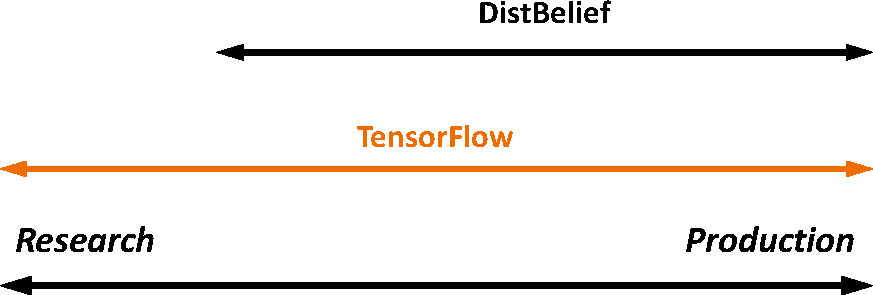
\includegraphics[width=.7\textwidth]{images/DistBeliefvsTensorFlow.pdf}\\
	\vspace{10pt} 
	\caption{Zielgruppenabdeckung von DistBelief und \gls{TF}~\cite{tf-sum17-keynote}}
	\label{fig:DBvsTF}
\end{figure}

\gls{TF} bietet zum einen genug Flexibilität für Forschungsprojekte, um mit neuen Modellen zu experimentieren, ist gleichzeitig aber hochperformant und robust, was beim Einsatz in Produktivsoftware wichtig ist. Modelle können somit also oft aus der Forschung direkt in Produktivumgebungen übernommen werden~\cite{tensorflow2016-whitepaper}.

\section{Datenflussgraphen in Tensorflow}
Einer der Hauptbestandteile für die Durchführung von Berechnungen mit \gls{TF} sind Datenflussgraphen~\cite{dataflow}, im Original "`dataflow graph"' genannt, welche aus einem oder mehreren Knoten bestehen~\cite{tensorflow2015-whitepaper}. Diese werden im Quellcode meist zu Beginn über eine der verfügbaren Client-Schnittstellen (Python oder C++) definiert und können bei Bedarf von TensorBoard dargestellt werden (\autoref{sub:tb-graph}). \autoref{lst:tf-graph} zeigt den Beispiel-Code für die Definition eines sehr einfachen Datenflussgraphen, bei dem zunächst in Zeile zwei ein Vektor \lstinline$b$ von der Größe 100 mit Nullen initialisiert wird. Anschließend wird in Zeile drei eine Matrix \lstinline$W$ mit den Dimensionen 625x100 mit Zufallswerten zwischen minus Eins und Eins belegt und in Zeile vier ein variabler Platzhalter \lstinline$x$ für die spätere Eingabe definiert. Der eigentliche Graph entsteht in Zeile fünf: Zunächst wird der Input \lstinline$x$ mit der Matrix \lstinline$W$ multipliziert und anschließend der Vektor \lstinline$b$ aufaddiert. Das Ergebnis wird abschließend einer ReLU-Funktion (\autoref{sub:relu}) übergeben. Diese Verkettung kann beliebig lange weitergeführt werden, was im Code in Zeile sechs und in der grafischen Darstellung in \autoref{fig:dataflow} durch den Platzhalter symbolisiert wird.

\begin{minipage}{\linewidth}
\begin{lstlisting}[language=Python, label=lst:tf-graph, caption={Code-Beispiel zur Definition eines Graphen~\cite{tensorflow2015-whitepaper}}]
import tensorflow as tf
b = tf.Variable(tf.zeros([100]))
W = tf.Variable(tf.random_uniform([625,100],-1,1))
x = tf.placeholder(name="x")
relu = tf.nn.relu(tf.matmul(W, x) + b)
C = [...]
\end{lstlisting}
\end{minipage}

\begin{figure}[htb!]
	\centering
	 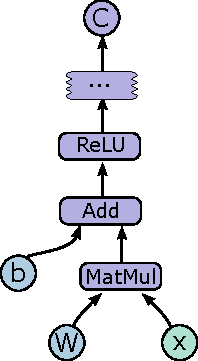
\includegraphics[width=.3\textwidth]{images/graph.pdf}\\
	\vspace{10pt} 
	\caption{Datenflussgraph zu \autoref{lst:tf-graph}~\cite{tensorflow2015-whitepaper}}
	\label{fig:dataflow}
\end{figure}

Jeder Knoten hat eine beliebige Anzahl an Ein- und Ausgängen und stellt eine Operation dar. Werte, die entlang normaler Kanten im Graph fließen (von Aus- zu Eingängen) werden "`Tensoren"' genannt, welche beliebig dimensionierten Arrays mit einem fest definierten Datentypen entsprechen. Des weiteren gibt es noch spezielle Kanten, genannt "`control dependencies"' über die keine Daten laufen. Diese indizieren, dass die Berechnungen im Quellknoten abgeschlossen sein müssen, bevor der Zielknoten starten kann. Somit können diese control dependencies verwendet werden um "`happens before"' Relationen zu implementieren, was zum Beispiel genutzt werden kann um den maximalen Speicherverbrauch zu kontrollieren.

\section{Hard- und Software Anforderungen}
Tensorflow wurde von Grund auf so gestaltet, dass es eine möglichst großen Bandbreite an Hardware zur Berechnung der \gls{NN} nutzen kann und auch größtenteils unabhängig von dem System ist, auf dem es ausgeführt wird.

\subsection{Betriebssysteme}
\gls{TF} ist seit dem Anfang auf Linux und MacOS lauffähig. Seit Version 0.12 wird außerdem Windows unterstützt~\cite{tf0.12}. Die reine Ausführung eines bereits trainierten Netzes (Inference) ist außerdem auch auf Android und iOS möglich~\cite{tensorflow2015-whitepaper}\cite{tensorflow2016-whitepaper}.

\subsection{Hardware Unterstützung}
Lernalgorithmen basieren oft auf aufwändigen Rechenoperationen, die zwar hoch parallelisierbar sind, meist jedoch auch große Abhängigkeiten beim Datenzugriff aufweisen. Ein Beispiel hierfür sind Matrix Multiplikationen. Mit dem Aufkommen von so genannten "`Generall Purpose GPUs"' die eine große Anzahl an Recheneinheiten und schnellen lokalen Speicher bieten, konnten \gls{NN} stark beschleunigt werden.

\gls{TF} bietet hier den Vorteil, dass es unabhängig von der vorhandenen Hardware eingesetzt werden kann. Es werden sowohl CPUs als auch eine Vielzahl von NVIDIA GPUs unterstützt. Im Moment können GPUs anderer Hersteller noch nicht genutzt werden, da gls{TF} die CUDA-API von NVIDIA nutzt. Diese "`CUDA Compute Capability"' muss von der Hardware auch mindestens in Version 3.0 unterstützt werden. Eine Liste mit allen unterstützen Karten kann auf der \href{https://developer.nvidia.com/cuda-gpus}{NVIDIA Homepage} gefunden werden~\cite{tfinstall}.

Neben diesen allgemein gehaltenen Recheneinheiten kann \gls{TF} auch spezielle Hardware für die Berechnungen nutzen. So gibt es von Google selbst sogenannte \glspl{TPU}, die eine enorme Beschleunigung von Inference ermöglichen und dabei vor allem wesentliche energieeffizienter sind, als CPUs oder auch GPUs~\cite{TPU}. Da es sich hierbei jedoch um proprietäre Hardware handelt, können diese \glspl{TPU} im Moment nur als Service in der Google Cloud genutzt werden~\cite{TPU2}. Außerdem kann der sogenannte "`Neural Compute Stick"' von Movidius (inzwischen Intel)~\cite{movidius} verwendet werden, der es auch auf leistungsschwacher Hardware wie zum Beispiel einem Raspberry Pi möglich macht, Inference von \gls{NN} durchzuführen.

In Tensorflow kann genau definiert werden, welche Schritte im Programmcode von welcher Recheneinheit ausgeführt werden sollen. So wird in Zeile zwei von \autoref{lst:tf-dev} angegeben, dass die dritte GPU im System verwendet werden soll\footnote{\gls{TF} beginnt bei null zu zählen}~\cite{tf-dev}.

\begin{minipage}{\linewidth}
\begin{lstlisting}[language=Python, label=lst:tf-dev, caption={Festlegung des Geräts, auf dem die Berechnung getätigt werden soll}]
# Creates a graph.
with tf.device('/device:GPU:2'):
  a = tf.constant([1.0, 2.0, 3.0, 4.0, 5.0, 6.0], shape=[2, 3], name='a')
  b = tf.constant([1.0, 2.0, 3.0, 4.0, 5.0, 6.0], shape=[3, 2], name='b')
  c = tf.matmul(a, b)
# Creates a session with log_device_placement set to True.
sess = tf.Session(config=tf.ConfigProto(log_device_placement=True))
# Runs the op.
print(sess.run(c))
\end{lstlisting}
\end{minipage}

In den Zeilen drei und vier werden zwei konstante Arrays definiert und in Zeile fünf wird die durchzuführende Rechenoperation festgelegt. In Zeile sieben wird eine TensorFlow Session erstellt und mit "`sess.run"' in Zeile neun wird schließlich die Berechnung angestoßen.

\subsection{Software Anforderungen}
\Gls{TF} ist sowohl unter Python 2.7 als auch unter Python 3 ab Version 3.4~\cite{tfinstall} lauffähig. Alternativ sind aber auch Docker Images verfügbar.

Für die Verwendung von NVIDIA GPUs muss außerdem das CUDA® Toolkit in Version 8.0 	sowie cuDNN v6.0 installiert werden~\cite{tfinstall}.

\section{Architektur von TensorFlow}
\Gls{TF} wurde als erweiterbare, plattformübergreifende Bibliothek konzipiert. \autoref{fig:architektur} zeigt, wie dies durch Modularisierung erreicht wurde. Dabei wird alles oberhalb der C-API als "`user-level"' bezeichnet und alles darunter als "`core library"'~\cite{tensorflow2016-whitepaper}.

\begin{figure}[htb!]
	\centering
	 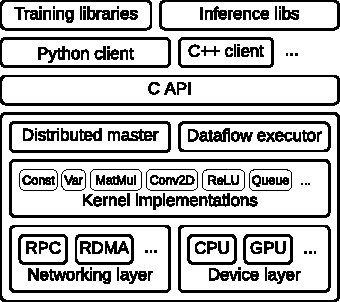
\includegraphics[width=.5\textwidth]{images/architektur.pdf}\\
	\vspace{10pt} 
	\caption{Die Architektur von \gls{TF}~\cite{tensorflow2016-whitepaper}}
	\label{fig:architektur}
\end{figure}

Die meisten Nutzer werden \gls{TF} über die bereitgestellten Client-Schnittstellen nutzen. Diese sind für die beiden Sprachen "`Python"' und "`C++"' vorhanden. Beide nutzen dabei eine C API, die den Zugriff auf die core-library von \gls{TF} ermöglicht. Diese wiederum wurden in C++ implementiert um Portabilität und Leistungsfähigkeit zu gewährleisten. Im user-level befinden sich außerdem noch Training- und Inference-Bibliotheken, in denen häufig genutzte Funktionen wie Backpropagation oder das Gradientenabstiegsverfahren aus
%%TODO ref!!
Kapitel 2.6 bereits implementiert wurden.

Der Kern von \gls{TF} besteht aus mehreren Komponenten. Der sogenannte "`distributed master"' teilt den Berechnungsgraphen in mehrere Sub-Graphen auf, die dann auf den einzelnen Recheneinheiten vom "`dataflow executor"' ausgeführt werden. Des weiteren sind mehr als 200 Standard-Operationen für zum Beispiel Array Manipulation oder Zustandsmanagement enthalten. Dabei wurde an vielen Stellen auf bereits bestehende Open-Source-Software aufgebaut, die eine effiziente Parallelberechnung auf Mehrkern-CPUs und GPUs sicherstellt.

Im "`Networking layer"' wurden erweiterte Netzwerkprotokolle wie "`gRPC over TCP"' oder "`RDMA over Converged Ethernet"' integriert, die eine schnelle Kommunikation zwischen entfernten Rechnern sicherstellen sollen. Doch auch innerhalb eines Rechners wurden zusätzliche Funktionen implementiert, die einen schnellen Datenaustausch von zum Beispiel zwei GPUs ermöglichen sollen.

\section{Nutzung von Tensorflow mit Keras}

Keras ist eine in Python geschriebene Bibliothek speziell zum Erstellen von \gls{NN}, die \gls{TF}, CNTK~\footnote{CNTK ist ein Deep-Learning Toolkit von Microsoft} oder Theano~\footnote{Theano ist eine Bibliothek für nummerische Berechnungen und wurde zu großen Teilen von der Universität Montreal entwickelt} als Backend für die Berechnungen verwenden kann. Der Fokus liegt dabei auf der schnellen Umsetzung von experimentellem Code und Unterstützung beim Prototyping~\cite{keras}. Hauptsächlich wird Keras von Google entwickelt, Teile jedoch auch von Microsoft, Amazon, NVIDIA und Weiteren. Keras wurde mit Versions 1.4 auch direkt in \gls{TF} integriert~\cite{tfRelease}.

In \autoref{lst:keras} (Anhang) ist Beispiel-Code für das Trainieren eines Models auf dem MNIST-Datenset zu finden. Am interessantesten sind hier die Zeilen 21--27, in denen das Model definiert wird. Zunächst wird in Zeile 21 festgelegt, dass ein Sequentielles Modell erstellt werden soll. Nachfolgend kann man die einzelnen Layer jeweils mit der \lstinline$.add$ Funktion hinzufügen. So werden in den Zeilen 22--24 drei sogenannte Dense- oder Fully-Connected-Layer definiert, bei denen jeweils jeder Knoten eine Kante zu jedem Knoten der übergeordneten Schicht besitzt. Bei den ersten beiden wird als Aktivierungsfunktion wieder die "`relu"' Funktion verwendet, bei der letzten kommt eine Softmax-Funktion zum Einsatz, die Wahrscheinlichkeiten auf die einzelnen Klassen aufteilt und somit bestimmt, welches Ergebnis ausgegeben wird. Der Code zeigt, wie einfach und vor allem intuitiv ein Model mit Hilfe von Keras erstellt werden kann.